\documentclass[12pt]{article}
 
\usepackage[margin=1in]{geometry} 
\usepackage{amsmath,amsthm,amssymb,outlines}
\usepackage{graphicx}
\usepackage{tikzsymbols}
\newenvironment{statement}[2][Statement]{\begin{trivlist}
\item[\hskip \labelsep {\bfseries #1}\hskip \labelsep {\bfseries #2.}]}{\end{trivlist}}

\begin{document}
 
\title{MATH 8150 Homework 2} 
\author{Dahlen Elstran} 
\maketitle

\begin{statement}[Problem]{(Stein) 2}
  Show that 
  \begin{align*}
    \int^{\infty}_0 \frac{\sin(x)}{x} dx=\frac{\pi}{2}.
  \end{align*}
\end{statement}
\begin{proof}
  First, consider the following function $f(z)=\frac{e^{iz}}{z}$ and contour $\gamma$:
    \begin{center} 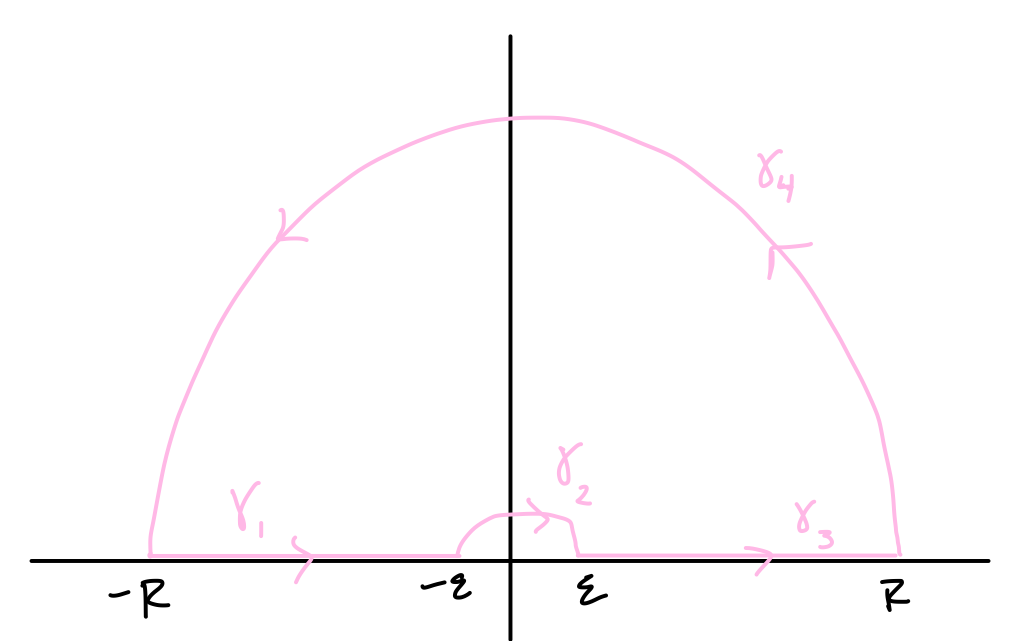
\includegraphics[scale=.2]{2-1.png} \end{center}
  Because the function is holomorphic on the closed contour, we can apply Cauchy's theorem to find that 
  \begin{equation*}
    \oint_{\gamma} f(z)dz = \int_{\gamma_1} f(z)dz + \int_{\gamma_2} f(z)dz + \int_{\gamma_3} f(z)dz +\int_{\gamma_4} f(z)dz = 0.
  \end{equation*}
  First, we evaluate the integrals over real numbers:
  \begin{equation*}
    \int_{\gamma_1} f(z)dz + \int_{\gamma_3} f(z)dz = \int_{-R}^{-\varepsilon} f(z)dz + \int_{\varepsilon}^{R} f(z)dz
  \end{equation*}
  Using u-subsitution and switch variables, we get 
  \begin{align*}
    \int^R_{\varepsilon} \frac{e^{ix}}{x}dx - \int^R_{\varepsilon} \frac{e^{-ix}}{x}dx &= \int^R_{\varepsilon} \frac{e^{ix}-e^{-ix}}{x}dx \\
                                                                                       &= 2i \int^R_{\varepsilon} \frac{e^{ix}-e^{-ix}}{(2i)x}dx \\
                                                                                       &= 2i \int^R_{\varepsilon} \frac{\sin (x)}{x}dx \\
                                                                                       & \to 2i \int^{\infty}_0 \frac{\sin (x)}{x}dx \text{ as } R \to \infty \text{ and } \varepsilon \to 0.
  \end{align*}
  Next, we evaluate the $\gamma_2$ integral with the following parametrization: 
  \begin{align*}
    z &=\gamma (t)= \varepsilon e^{i(\pi - t)} \text{ where } t \in [0,\pi]\\
    dz &= \gamma '(t)dt \\ 
       &= -i \varepsilon e^{i(\pi - t)} dt \\
       &= -i \gamma (t) dt
  \end{align*}
  So then
  \begin{align*}
  \int_{\gamma_2} \frac{e^{iz}}{z}dz &= \int^{\pi}_0 \frac{e^{i \gamma (t)}}{\gamma (t)}dt \\
                                     &= -i \int^{\pi}_0 e^{i \gamma (t)}dt \\
                                     &= -i \int^{\pi}_0 e^{i \varepsilon e^{i (\pi - t)}}dt
  \end{align*}
  As $\varepsilon \to 0$, this approaches 
  \begin{equation*}
    -i \int^{\pi}_0 1 \cdot dt = -i \pi.
  \end{equation*}
  For the last integral, use the following parametrization:
  \begin{align*}
    z &= \gamma(t)=Re^{it} \\
    dz &= \gamma ' (t)dt \\
       &= Re^{it}dt \\
       &= \gamma (t) dt
  \end{align*}
  So we have 
  \begin{align*}
    \int_{\gamma_4} f(z)dz &= \int^{\pi}_0 \frac{e^{i \gamma (t)}}{\gamma (t)} \gamma (t) dt \\
                           &= \int^{\pi}_0 e^{i \gamma (t)} dt \\
                           &= \int^{\pi}_0 e^{iRe^{it}} dt \\
                           &= \int^{\pi}_0 e^{iR(\cos (t) + i \sin (t))}dt. 
  \end{align*}
  Then note that 
  \begin{align*}
    \left\lvert \int^{\pi}_0 e^{iR(\cos (t) + i \sin (t))}dt \right\rvert & \leq \int^{\pi}_0 \left\lvert e^{iR(\cos (t) + i \sin (t))} \right \rvert dt \\
                                                                        &= \int^{\pi}_0 \left \lvert e^{iR\cos(t)} \right\rvert \left\lvert e^{-R\sin(t)}\right\rvert dt \\
                                                                        &= \int^{\pi}_0 1 \cdot \left\lvert e^{-R\sin(t)} \right\rvert dt \\
                                                                        &= \int^{\pi}_0 e^{-R\sin(t)}dt \\
                                                                        & \to 0 \text{ as } R \to \infty .
  \end{align*}
  So we find that this integral must be 0.
  Finally, we have 
  \begin{align*} 
    \oint_{\gamma} f(z)dz &= \int_{\gamma_1} f(z)dz + \int_{\gamma_2} f(z)dz + \int_{\gamma_3} f(z)dz +\int_{\gamma_4} f(z)dz \\
                          &= 2i \int^{\pi}_0 \frac{\sin(x)}{x} dx - i\pi + 0 \\
                          &= 0.
  \end{align*}
  Thus, 
  \begin{equation*}
    \int^{\pi}_0 \frac{\sin(x)}{x} dx = \frac{\pi}{2}.
  \end{equation*}
\end{proof}

\begin{statement}[Problem]{(Tie) 2}
  Let $f$ be any power series centered at the origin. Prove that $f$ has a power series expansion around any point in it's disc of convergence.
\end{statement}
\begin{proof}
  By Cauchy's integral formula, we know that 
  \begin{equation*}
    f(z) = \int \frac{f(\xi)}{\xi - z} d \xi.
  \end{equation*}
  We can rearrange this to be
  \begin{equation*}
    \int f(\xi) \cdot \frac{1}{\xi - z + z_0 -z_0}
  \end{equation*}
  where $z_0$ is any point in the disc of convergence of $f$. 
  \par Let $w = \frac{z-z_0}{\xi - z_0}$ so that 
  \begin{equation*}
    \int \frac{f(\xi)}{\xi - z_0} \cdot \frac{1}{1-w} = \int \frac{f(\xi)}{\xi - z_0} \sum_{n \geq  0} w^n d \xi.
  \end{equation*}
  From here, we can bring the integral into the sum:
  \begin{equation*}
    \sum_{n \geq 0} \int \frac{f(\xi)}{\xi - z_0} d \xi \cdot w^n
  \end{equation*}
  Then note that 
  \begin{align*} 
    \sum_{n \geq 0} \int \frac{f(\xi)}{\xi - z_0} d \xi \cdot w^n &= \sum_{n \geq 0} \int \frac{f(\xi)}{\xi - z_0} d \xi \cdot \frac{(z-z_0)^n}{(\xi - z_0)^n} \\
                                                                  &= \sum_{n \geq 0} \int \frac{f(\xi)}{(\xi - z_0)^{k+1}} d \xi \cdot (z-z_0)^k
  \end{align*}
  Thus we are left with a power series centered at $z_0$, an arbitrary point in the disc of convergence.
\end{proof}

\begin{statement}[Problem]{(Tie) 3}
  Prove the following:
  \begin{itemize}
    \item[(a)] The power series $\sum^{\infty}_{n=1} nz^n$ does not converge at any point of the unit circle. 
    \item[(b)] The power series $\sum^{\infty}_{n=1} \frac{z^n}{n^2}$ converges at every point of the unit circle. 
    \item[(c)] The power series $\sum^{\infty}{n=1} \frac{z^n}{n}$ converges at every point of the unit circle except at $z=1$. 
  \end{itemize}
\end{statement}
\begin{proof}
  \begin{itemize}
    \item[(a)] If the point is on the unit circle, we know that $\lvert z \rvert = 1$. Thus 
      \begin{equation*} 
        \lvert nz^n \rvert = \lvert n \rvert \to \infty.
      \end{equation*}
      so that the series does not converge. 
    \item[(b)] Because 
      \begin{align*}
        \left\lvert \sum \frac{z^n}{n^2} \right\rvert & \leq \sum \left\lvert \frac{z^n}{n^2} \right\rvert \\
                                                      &= \sum \left\lvert \frac{1}{n^2} \right\rvert \cdot \left\lvert z^n \right\rvert \\
                                                      &= \sum \left\lvert \frac{1}{n^2} \right\rvert \\
                                                      & < \infty,
      \end{align*}
      we know the series converges absolutely, which implies convergence. 
    \item[(c)]
  \end{itemize}
\end{proof}

\begin{statement}[Problem]{(Tie) 4} 
  Don't use the Cauchy integral formula. Show that if $\lvert a \rvert < r < \lvert b \rvert$, then 
  \begin{equation*}
    \int_{\gamma} \frac{dz}{(z-\alpha)(z-\beta)} = \frac{2\pi 1}{\alpha - \beta}
  \end{equation*}
  where $\gamma$ denotes the circle centered at the origin, of radius $r$, with positive orientation. 
\end{statement}
\begin{proof}
  First, we can rewrite the integral like so using partial fractions:
  \begin{equation*}
    \int_{\gamma} \frac{dz}{(z-\alpha)(z-\beta)} = \frac{1}{a-b} \left (\int_{\gamma} \frac{dz}{z-a} - \int_{\gamma} \frac{dz}{z-b} \right )
  \end{equation*}
  Then because $\alpha$ is inside $\gamma$, we can say 
  \begin{equation*}
    \int_{\gamma} \frac{dz}{z-\alpha} = 2\pi i.
  \end{equation*}
  Similarly, because $\beta$ is outside $\gamma$, we know 
  \begin{equation*}
    \int_{\gamma} \frac{dz}{z-\beta} = 0
  \end{equation*}
  Thus 
  \begin{equation*}
    \int_{\gamma} \frac{dz}{(z-\alpha)(z-\beta)} = \frac{2\pi 1}{\alpha - \beta}.
  \end{equation*} 
\end{proof}

\par Note: I started this assignment way too late, I have definitely learned my lesson :(

\end{document}
